% !TEX root = CSUR/main.tex

\section{Introduction}

Symbolic execution is a very powerful static analysis technique introduced in the mid 70's to perform software testing (see, e.g.,~{\cite{K-CACM76} and~\cite{H-TSE77}})\mynote{IF: are references appropriate? Should we give more credits? It seems several groups introduced independently this technique}. The basic idea is to allow the program to take on ``symbolic'' -- instead of concrete -- input values and to associate variables with expressions and constraints in terms of those symbols during a symbolic execution of the program itself. In this paper we survey the main aspects of symbolic execution and discuss its extensive usage in the context of computer security for analyzing programs at the level of both source and binary code.

\paragraph{Black-box approach versus white-box approach}

Discussion\mynote{IF: do we really need this?} of black-box approach and white-box approach. Symbolic execution is a white-box technique. Black-box approaches can be very fast but not always effective. White-box approaches can be very effective but are typically slower than black-box techniques. An in-depth discussion of this aspect will be done when we will discuss~\cite{DRILLER-NDSS16}.

\begin{figure}[H]
  \vspace{-3mm}
  \centering
  \begin{subfigure}{.5\textwidth}
    \centering
    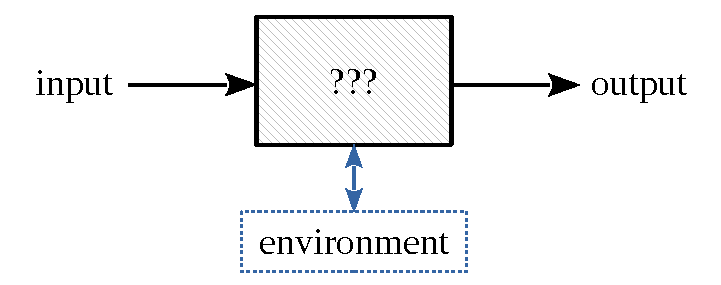
\includegraphics[width=0.9\linewidth]{images/blackbox} 
    \caption{Black-box approach}
    %\label{fig:sub1}
  \end{subfigure}%
  \begin{subfigure}{.5\textwidth}
    \centering
    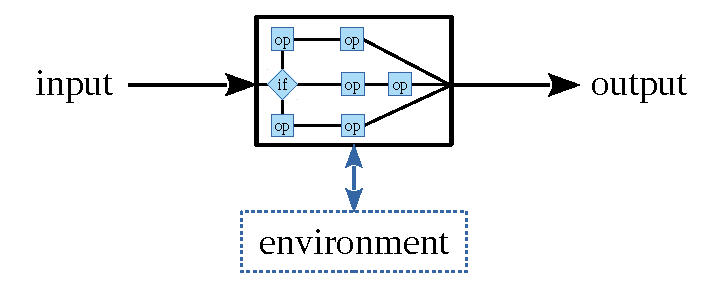
\includegraphics[width=0.9\linewidth]{images/whitebox} 
    \caption{White-box approach}
    %\label{fig:sub2}
  \end{subfigure}
  %\label{fig:example-symbolic-execution}
  \vspace{-3mm}
\end{figure}
